\documentclass{article}
\usepackage{graphicx} % Required for inserting images
\usepackage{amsmath,amssymb,amsthm}
\usepackage{graphicx,float}
\graphicspath{{images/}}
\usepackage[none]{hyphenat}
\usepackage{blindtext}
\usepackage{parskip}
\usepackage[letterpaper,top=3cm, left= 3cm,bottom=3cm]{geometry}
\DeclareMathOperator{\arcsec}{arcsec}
\DeclareMathOperator{\arccot}{arccot}
\DeclareMathOperator{\arccsc}{arccsc}
\usepackage{subcaption}

\title{Trigonometric Functions}
\author{Polaris}
\date{October 2024}

\begin{document} 

\maketitle

\section{Definition}
\begin{figure}[H]
    \centering
    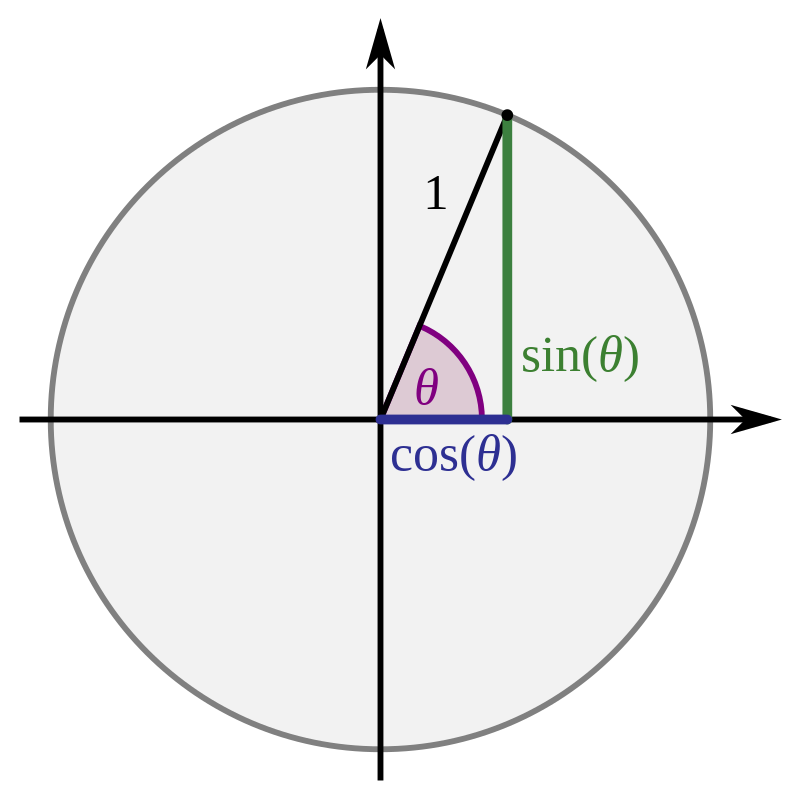
\includegraphics[width = 8cm]{pictures/trig.png}
    \caption{Defining trig functions in a unit circle}
\end{figure}


\section{Trigonometric Identities}
\subsection{Pythagorean Identities}
\begin{equation}
    \sin^2 x + \cos^2 x =1
\end{equation}
\begin{equation}
    1 + \tan^2 x = \sec^2 x
\end{equation}
\begin{equation}
    1 + \cot^2 x = \csc^2 x
\end{equation}

\subsection{Angle Sum and Difference}
\begin{equation}
    \sin(x+y) = \sin x \cos y + \cos x \sin y
\end{equation}
\begin{equation}
    \sin(x-y) = \sin x \cos y - \cos x \sin y
\end{equation}
\begin{equation}
    \cos(x+y) = \cos x \cos y - \sin x \sin y
\end{equation}
\begin{equation}
    \cos(x-y) = \cos x \cos y + \sin x \sin y
\end{equation}

\subsection{Product to Sum}
\begin{equation}
    \sin x \sin y = \frac{1}{2}(\cos(x-y)-\cos(x+y))
\end{equation}
\begin{equation}
    \cos x \cos y = \frac{1}{2}(\cos(x+y)+\cos(x-y))
\end{equation}
\begin{equation}
    \sin x \cos y = \frac{1}{2}(\sin(x+y)+\sin(x-y))
\end{equation}

\subsection{Sum to Product}
\begin{equation}
    \sin x + \sin y = 2 \sin(\frac{x+y}{2})\cos(\frac{x-y}{2})
\end{equation}
\begin{equation}
    \sin x + \sin y = 2 \sin(\frac{x-y}{2})\cos(\frac{x+y}{2})
\end{equation}
\begin{equation}
    \cos x + \cos y = 2 \cos(\frac{x+y}{2}) \cos(\frac{x-y}{2})
\end{equation}
\begin{equation}
    \cos x - \cos y = 2 \sin(\frac{x+y}{2})\sin(\frac{x-y}{2})
\end{equation}

\subsection{Double Angle Formula}
\begin{equation}
    \sin (2x) = 2 \sin x \cos x
\end{equation}
can be derived from (1.4)
\begin{equation}
    \cos 2x = \cos^2x-\sin^2x
\end{equation}
can be derived from (1.6)

\subsection{Half Angle formula}
\begin{equation}
    \sin \frac{x}{2} = \sqrt{\frac{1 + \cos x}{2}}
\end{equation}
The sign of $\sqrt{\frac{1 + \cos x}{2}}$ is the same as $\sin \frac{x}{2}$.
\begin{equation}
    \cos \frac{x}{2} = \sqrt{\frac{1 + \cos x}{2}}
\end{equation}
The sign of $\sqrt{\frac{1 + \cos x}{2}}$ is the same as $\cos \frac{x}{2}$

\subsection{Power Reduction Formula}
\begin{equation}
    \sin^2x = \frac{1 - \cos 2x}{2}
\end{equation}
\begin{equation}
    \cos^2x = \frac{1 + \cos 2x}{2}
\end{equation}

\subsection{Linear Combination of Sine and Cosine}
\begin{equation}
    a\sin x + b\cos x = c\cos (x + \varphi)
\end{equation}
where: $c = \text{sgn}(a)\sqrt{a^2+b^2}$, $\tan \varphi = \frac{b}{a}$

\newpage
\section{Limits of Trig Functions}
\[
    \lim_{x\to 0} \frac{\sin x }{x} = 1
\]
First let's see this in a graph, let $f(x) = \sin x$, $g(x) = x$ the graph of the two functions are:
\begin{figure}[H]
    \centering
    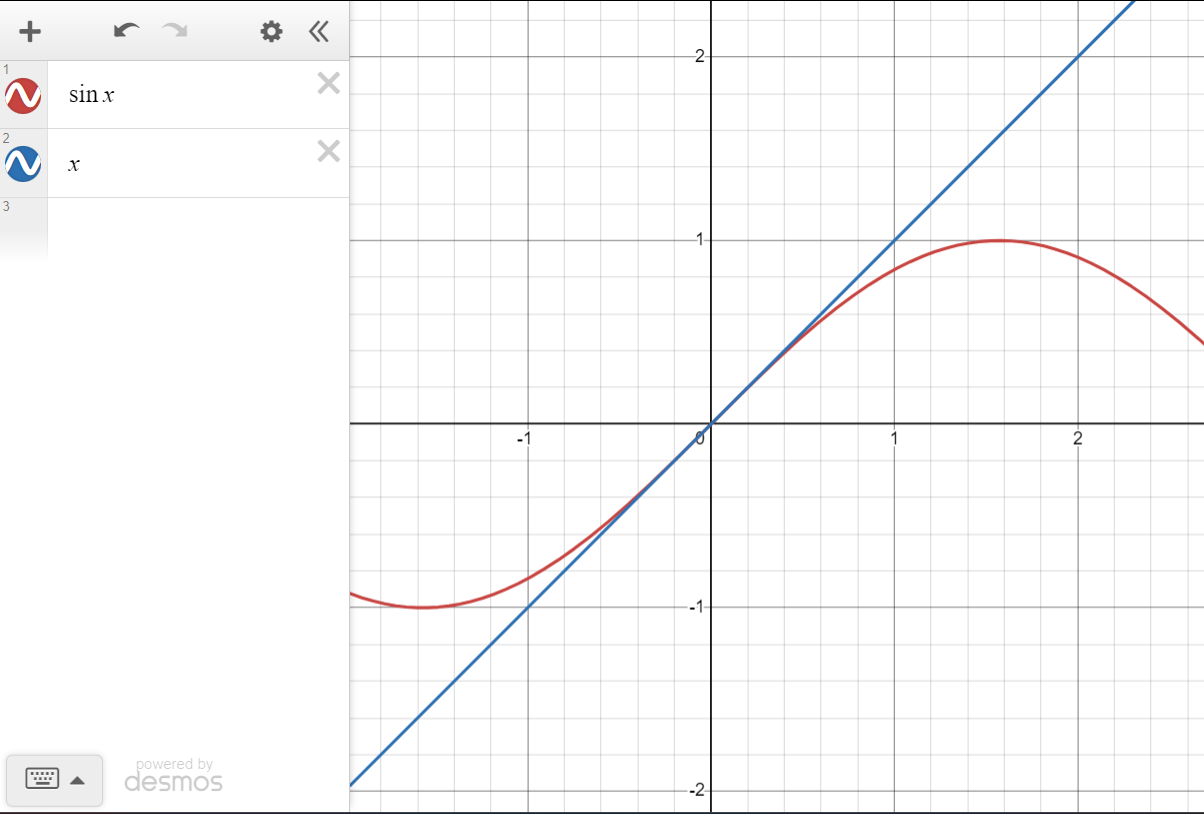
\includegraphics[width = 12cm]{pictures/triglimit1.png}
    \caption{Graph of $\sin x$ and $x$ around 0}
\end{figure}
Now from this graph, we can see that the two functions are equal in $x=0$, therefore we can assume that the limit is 1 (limit is not equal, the function is not defined at $x=0$)

To prove this limit, we will use the squeeze theorem, which is:
\begin{center}
    In an interval $I$ that contains the point $a$, let $f, g, h$ be 3 functions that is defined in the interval $I$, but not necessarily in $a$, if three functions satisfy:

    $f(x) \leq g(x) \leq h(x)$
\end{center}
also suppose that
    \[
    \lim_{x\to a} f(x) = L, \lim_{x\to a} h(x) = L
    \]
then
    \[
    \lim_{x\to a } g(x) = L
    \]
\newpage
With this prepare, we can prove this very important limit:
\begin{figure}[H]
    \centering
    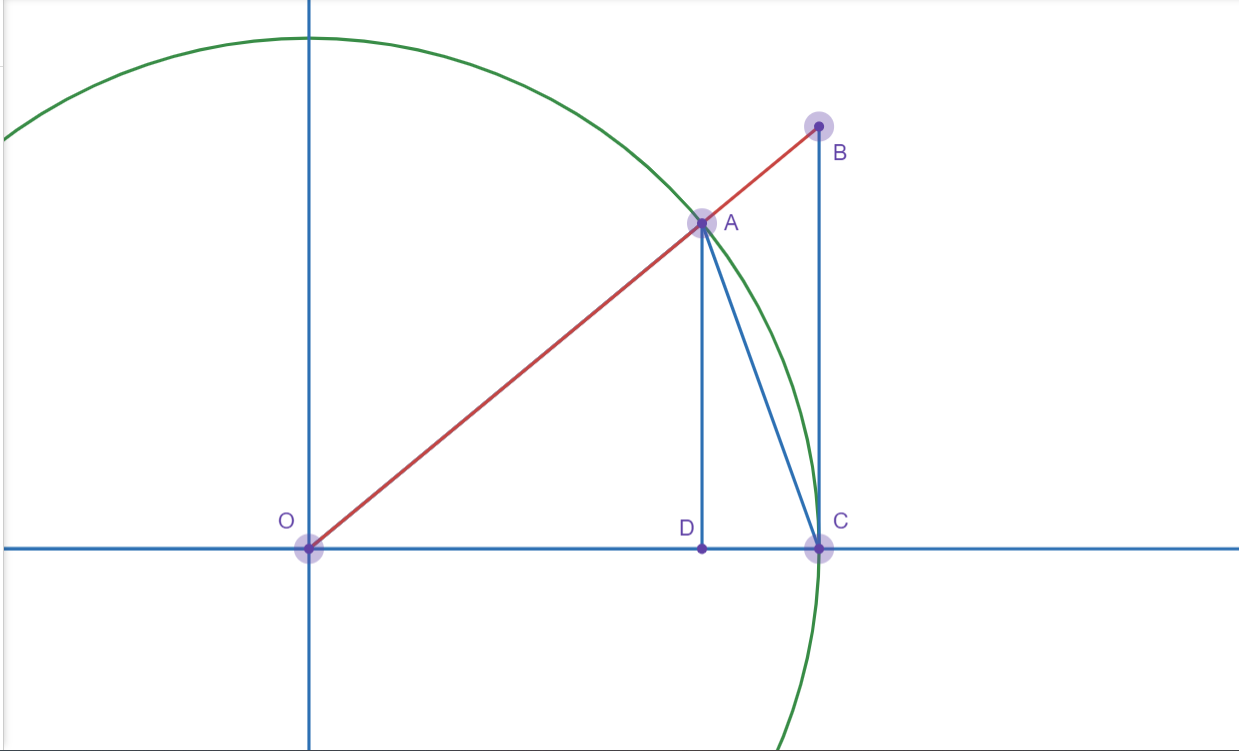
\includegraphics[width = 12cm]{pictures/triglimit2.png}
\end{figure}
In this diagram:
$\begin{cases}
    x = \angle AOC\\
    OD = \cos x\\
    AD = \sin x\\
    BC = \tan x 
\end{cases}$, also notice that $S_{\triangle AOC} \leq S_{\text{circular sector} AOC} \leq S_{\triangle BOC}$

We arrive at this inequalities:
\begin{equation}
    \frac{1}{2}\sin x \leq \frac{1}{2} x \leq \frac{1}{2}\frac{\sin x}{\cos x}
\end{equation}
Divide $\sin x$ and $\frac{1}{2}$ from both sides, we get:
\[
    1 \leq \frac{x}{\sin x} \leq \frac{1}{\cos x}
\]
or 
\[
    1 \leq \frac{\sin x}{x} \leq \cos x
\]
If we take limit to 0 from both sides, we get:
\[
    \lim_{x\to 0} 1 \leq \lim_{x\to 0}\frac{\sin x}{x} \leq \lim_{x\to 0} \cos x
\]
By squeeze theorem, we get:
\begin{equation}
    \lim_{x\to 0} \frac{\sin x }{x} = 1
\end{equation}

\newpage
Another limit we are interested in is 
\[
    \lim_{x\to 0}\frac{1-\cos x}{x} = 0
\]
This limit can be proved algebraically, we can multiply both side by $1+\cos x$, the limit becomes:
\[
    \lim_{x\to 0}\frac{(1-\cos x)(1+\cos x)}{x(1+\cos x)}
\]
which can be rearranged to
\[
    \lim_{x\to 0}\frac{\sin x}{x}\frac{1}{1+\cos x}\sin x
\]
Then substitute the values in, it is easy to see that the limit of this function is:
\begin{equation}
    \lim_{x\to 0}\frac{1-\cos x}{x} = 0
\end{equation}

\section{Derivative of Trig functions}
By the definition of derivatives, it is easy to find the derivatives of $\sin x$ and $\cos x$
\subsection{sin}
The definition of derivatives:
\begin{equation}
    f'(x) = \lim_{h\to 0}\frac{f(x+h)-f(x)}{h}
\end{equation}
First, we will start with sin:
\[
    \frac{d}{dx}\sin x = \lim_{h\to 0 }\frac{\sin(x+h)-\sin x}{h}
\]
Recall (2.4), we see that:
\[
    \frac{d}{dx}\sin x = \lim_{h\to 0}\frac{\sin x \cos h + \cos x \sin h - \sin x}{h}
\]
which can be rearranged into:
\[
    \frac{d}{dx}\sin x = \lim_{h\to 0}\frac{\sin x \cos h -\sin x}{h} + \lim_{h\to 0} \frac{\cos x \sin h}{h}
\]
\[
    \frac{d}{dx}\sin x = \lim_{h\to 0}\frac{\sin x (\cos h - 1)}{h} + \lim_{h\to 0} \frac{\cos x \sin h}{h}
\]
By (3.2) and (3.3), we arrive at the derivative of sin:
\begin{equation}
    \frac{d}{dx}\sin x = \cos x
\end{equation}

\subsection{cos}
Using similar methods, we can also find the derivative of cosine function:
\[
    \frac{d}{dx}\cos x = \lim_{h\to 0}\frac{\cos(x+h) - \cos h}{h}
\]
Recall (2.6):
\[
    \frac{d}{dx}\cos x = \lim_{h\to 0}\frac{\cos x\cos h - \sin x \sin h - \cos h}{h}
\]
\[
    \frac{d}{dx}\cos x = \lim_{h\to 0}\frac{\cos x (\cos h -1)}{h} - \lim_{h\to 0}\frac{\sin x \sin h}{h}
\]
By (3.2) and (3.3), the derivative of cos is:
\begin{equation}
    \frac{d}{dx}\cos x = -\sin x
\end{equation}

\subsection{tan, csc, sec, cot}
All of these functions can be expressed using $\sin x$ and $\cos x$:
$\begin{cases}
    \tan x = \frac{\sin x}{\cos x}\\
    \csc x = \frac{1}{\sin x}\\
    \sec x = \frac{1}{\cos x}\\
    \cot x = \frac{1}{\tan x} = \frac{\cos x}{\sin x}
\end{cases}$

We can use quotient law to differentiate the functions:
\begin{equation}
    (\frac{u}{v})' = \frac{u'v - v'u}{v^2}
\end{equation}
For $\tan x$, it will be:
\[
    \frac{d}{dx} = \frac{d}{dx}\frac{\sin x}{\cos x} = \frac{(\sin x)' \cos x - (\cos x)' \sin x}{\cos^2 x}
\]
Note that $(\sin x)' = \cos x$, $(\cos x)' = -\sin x$, we get:
\[
    \frac{d}{dx}\tan x = \frac{\cos^2 x + \sin^2 x}{\cos^2 x}
\]
Which finally gives the result of:
\begin{equation}
    \frac{d}{dx} \tan x = \frac{1}{\cos^2 x} = \sec^2 x
\end{equation}
Using similar methods, we can get the derivative of $\csc x$, $\sec x$ and $\cot x$:
\begin{equation}
    \frac{d}{dx} \csc x = -\csc x \cot x = -\frac{\cos x}{\sin^2 x}\\
\end{equation}
\begin{equation}
    \frac{d}{dx} \sec x = \sec x \tan x = \frac{\sin x}{\cos^2 x}\\
\end{equation}
\begin{equation}
    \frac{d}{dx} \cot x = -\csc^2 x = -\frac{1}{\sin^2 x}
\end{equation}
The proof is an exercise left for the readers.

\subsection{arcsin, arccos, arctan}
Another interesting type of function we will examine is inverse trig functions, we will first introduce the inverse funtcion theorem:

If a function $x = f(y)$ is monotonic, differentiable and $f'(y) \neq 0$, its inverse function $y = f^{-1}(x)$ is also differentiable, thus:
\begin{equation}
    [f^{-1}(x)]' = \frac{1}{f'(y)} \text{ or } \frac{dy}{dx} = \frac{1}{\frac{dx}{dy}}
\end{equation}

It can be simplified into one sentence: the derivative of the inverse function is the reciprocal of the derivative of the original function

This theorem looks wordy and boring, so we will get the feel of it with some examples.

\newpage
Consider $y = \arcsin x$, its inverse function is $x = \sin y$, let's differentiate $x = \sin y$:
\[
    \frac{dx}{dy} = \frac{d}{dy}\sin y = \cos y
\]
By inverse function theorem:
\[
    \frac{dy}{dx} = \frac{d}{dx}\arcsin x = \frac{1}{\cos y }
\]
Notice that $\cos y = \sqrt{1-\sin^2 y} = \sqrt{1 - x^2}$, we arrived at the derivative of $\arcsin x$:
\begin{equation}
    \frac{d}{dx}\arcsin x = \frac{1}{\sqrt{1-x^2}}
\end{equation}

For $y = \arccos x$, its inverse function is $x = \cos y$:
\[
    \frac{dx}{dy} = \frac{d}{dy} \cos y = -\sin y
\]
By inverse function theorem:
\[
    \frac{dy}{dx} = \frac{d}{dx}\arccos x = -\frac{1}{\sin y}
\]
Notice that $\sin y = \sqrt{1-\cos^2 y}$, we arrived at the derivative of $\arccos x$

\begin{equation}
    \frac{d}{dx}\arccos x = -\frac{1}{\sqrt{1-x^2}}
\end{equation}

Notice that these two derivatives look very alike, which leads us to a property of $\arcsin x$ and $\arccos x$:
\begin{equation}
    \arcsin x + \arccos x = \frac{\pi}{2}
\end{equation}
This is because:
\[
    \frac{d}{dx}\arcsin x + \frac{d}{dx}\arccos x = 0
\]
and a derivative of 0 means a constant, namely $\frac{\pi}{2}$, it is very easy to work it out.

For $y = \arctan x$, its inverse function is $x = \tan y$, differentiate this function and we got:
\[
    \frac{dx}{dy} = \frac{d}{dy} \tan y = \sec^2 y
\]
\[
    \frac{dy}{dx} = \frac{d}{dx} \arctan x = \frac{1}{\sec^2 y}
\]
Notice that $1+\tan^2 y = \sec^2 y$, which gives:
\begin{equation}
    \frac{d}{dx} \arctan x = \frac{1}{1+x^2}
\end{equation}
\newpage
\section{Integral of trig functions}
We will start with the basic functions:
\subsection{Indefinite integral of trig functions}

\subsubsection{Simple Indefinite Integral}
\begin{equation}
    \int \cos x dx = \sin x + C
\end{equation}
\begin{equation}
    \int \sin x dx = -\cos x + C
\end{equation}
\begin{equation}
    \int \sec^2 x dx = \tan x + C
\end{equation}
\begin{equation}
    \int \frac{1}{\sqrt{1-x^2}} dx = \arcsin x + C
\end{equation}
\begin{equation}
    \int \frac{1}{1+x^2} dx = \arctan x + C
\end{equation}
\[
    \int \tan x dx
\]
We can split $\tan x = \frac{\sin x}{\cos x}$, which gives:
\[
    \int \frac{\sin x}{\cos x} dx= \int -\frac{1}{\cos x} d(\cos x)
\]
Which leads to our answer:
\begin{equation}
    \int \tan x dx = -\ln|\cos x| + C
\end{equation}

\subsubsection{Using Pythagorean Identities}
The following integrals will use some trig identities
\[
    \int \sin^3 x dx
\]
Use the trig identity of $\sin^2 x + \cos^2 = 1$, we get:
\[
    \int (1 - \cos^2 x) \sin x dx = \int (1 - \cos^2 x) d(\cos x) = -\int d(\cos x) + \int \cos^2 x d(\cos x)
\]
Which leads to our answer:
\begin{equation}
    \int \sin^3 x dx = -\cos x + \frac{1}{3}\cos^3 x + C
\end{equation}
Another example we will examine is:
\[
    \int \sec^6 x dx
\]
Notice that $1 + \tan^2 x = \sec^2 x$:
\[
    \int \sec^4 x \sec^2 x dx = \int (1 + \tan^2 x)^2 d(\tan x) = \int (1 + 2\tan^2 x + \tan^4 x)d(\tan x)
\]
Which leads to our answer:
\begin{equation}
    \int \sec^6 x = \tan x + \frac{2}{3}\tan^3 x + \frac{1}{5}\tan^5 x + C
\end{equation}

\newpage
\subsubsection{Using Power Reduction Formula}
\[
    \int \cos^2 x dx 
\]
By Power Reduction Formula: 
\[
    \cos^2 x = \frac{1 + \cos 2x}{2}
\]
the integrand can be rewritten as:
\[
    \int \frac{1 + \cos 2x}{2}dx = \int \frac{1}{2}dx + \int \frac{\cos 2x}{2\cdot 2} d(2x)
\]
Which leads to our answer:
\begin{equation}
    \int \cos^2 dx = \frac{1}{2} + \frac{1}{4} \sin 2x + C
\end{equation}

\[
    \int \sin^2 x dx
\]
By Power Reduction Formula:
\[
    \sin^2 x = \frac{1 - \cos 2x}{2}
\]
The integrand can be rewritten as:
\[
    \int \frac{1 - \cos 2x}{2} dx = \int \frac{1}{2} dx - \int \frac{\cos 2x}{2 \cdot 2} d(2x)
\]
Which leads to our answer:
\begin{equation}
    \int \sin^2 x dx = \frac{1}{2}x - \frac{1}{4} \sin 2x + C
\end{equation}

\subsubsection{Using Product to Sum }
\[
    \int \cos 3x \cos 2x dx
\]
By Product to Sum:
\[
    \cos x \cos y = \frac{1}{2}(\cos(x+y) + \cos(x-y))
\]
The integral can be written as:
\[
    \int \frac{1}{2}(\cos5x + \cos x)dx = \frac{1}{2\cdot 5} \int \cos 5x d(5x) + \frac{1}{2}\int \cos x dx
\]
Which gives the results:
\begin{equation}
    \int \cos 3x \cos 2x dx = \frac{1}{10} \sin 5x + \frac{1}{2} \sin x + C
\end{equation}

\newpage
\subsubsection{Integration by Parts with trig functions}
The formula for Integration by Parts is:
\begin{equation}
    \int u dv = uv - \int v du
\end{equation}
Let's start with an classic example:
\[
    \int x \sin x dx
\]
The integral can be written as:
\[
    \int x \sin x dx = - \int x d(\cos x ) = - x\cos x + \int \cos x dx
\]
Which leads to the result:
\begin{equation}
    \int x \sin x dx = -x \cos x + \sin x + C
\end{equation}

Using Integration by Parts, we can also find the integral of inverse trig function:
\[
    \int \arccos x dx
\]
Let $u = \arccos x$, $dv = du$, the integral can be written as:
\[
    \int \arccos x dx = x\arccos x - \int x d(\arccos x)\\
\]
\[
    = x\arccos x + \int x \frac{1}{\sqrt{1-x^2}}dx\\
\]
\[
    = x\arccos x - \frac{1}{2}\int \frac{1}{\sqrt{1-x^2}} d(1-x^2)
\]
\[
    = x\arccos x - \sqrt{1-x^2} + C
\]

\newpage
\subsubsection{Trig sub}
Note: this technique is sometimes tedious and annoying, don't use it unless its a must use.

Let's start with a simple example:

\[
    \int \sqrt{a^2-x^2}dx
\]
Note that there is a Pythagorean identity that looks awfully similar to this:
\[
    \sin^2 x + \cos^2 x = 1
\]
Hence let $x = a\sin t$, thus $dx = a \cos t dt$, substitute everything in:
\begin{equation} \nonumber
    \begin{split}
        \int \sqrt{a^2-x^2}dx & = \int \sqrt{a^2 - a^2\sin^2 t} \ a\cos t dt \\
        & = \int \sqrt{a^2(1-\sin^2 t)} \ a\cos t dt \\
        & = a^2 \int \cos^2 t dt \\
    \end{split}
\end{equation}
We already know how to integrate $\cos^2 t dt$, which makes our answer:
\[
    \int \sqrt{a^2-x^2}dx = \frac{a^2}{2} t + \frac{a^2}{2}\sin t \cos t +C
\]
Next we will substitute $x$ back, we know that $x = a\sin t$, hence $t = \arcsin x/a$:

\begin{equation}
    \int \sqrt{a^2-x^2}dx = \frac{a^2}{2} \arcsin \frac{x}{a} + \frac{1}{2} x \sqrt{a^2-x^2} +C
\end{equation}

Let's look at a similar example:
\[
    \int \frac{1}{\sqrt{x^2+a^2}}dx
\]
We can recall that:
\[
    1 + \tan^2 t = \sec^2 t
\]
Hence, let $x = a\tan t$, $dx = a \sec^2 t dt$, substitute everything in:
\begin{equation}\nonumber
    \begin{split}
        \int \frac{1}{\sqrt{x^2 + a^2}}dx &= \int \frac{1}{\sqrt{a^2 \tan^2 t + a^2}} a \sec^2 t dt \\
        & = \int \frac{1}{a\sqrt{1 + \tan^2 t}} a \sec^2 t dt \\ 
        & = \int \sec t dt \\
        & = \ln |\sec t + \tan t| + C\\
    \end{split} 
\end{equation}
Here we ran into a problem that we don't know what is $\sec t$ in terms of $x$, the simplest way is to draw an auxillary triangle:

\begin{figure}[H]
    \centering
    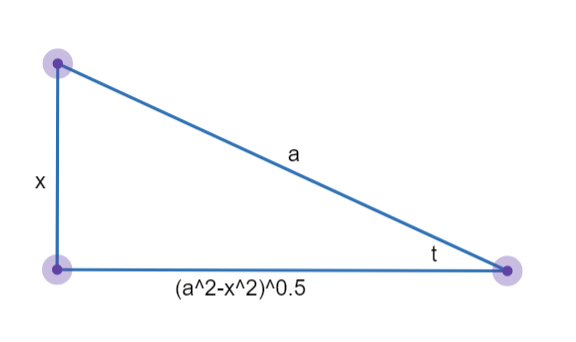
\includegraphics[width = 10cm]{pictures/trigsub.png}
\end{figure}

(Ignore the terrible handwriting), from this triangle, we can see that:
\[
    \sec t = \frac{\sqrt{a^2-t^2}}{a} \ \tan t = \frac{x}{a}\\
\]
Substitute them in, we get our final answer:
\begin{equation}
    \int \sqrt{a^2-x^2}dx = \ln(x+\sqrt{x^2+a^2}) + C
\end{equation}
Since $\ln(x/y) = \ln x - \ln y$, we put $\ln a$ as a constant and combined it into $+C$.

\subsection{Definite integral}
$f(x) = \sin x$ is an odd funtcion, so:
\begin{equation}
    \int_{-a}^{a} \sin x dx = 0
\end{equation}
$f(x) = \tan x$ is also an odd function, so:
\begin{equation}
    \int_{-a}^{a} \tan x dx = 0
\end{equation}
Wallis Equation:
\begin{equation}
    \int_0^{\frac{\pi}{2}} \sin^n x dx \ (\int_0^{\frac{\pi}{2}}\cos^n x dx) = 
\end{equation}
$\begin{cases}
    \frac{n-1}{n} \cdot \frac{n-3}{n-2} ...... \cdot \frac{3}{4} \cdot \frac{1}{2} \cdot \frac{\pi}{2} (\text{$n$ is a postive even integer})\\
    \frac{n-1}{n} \cdot \frac{n-3}{n-2} ...... \cdot \frac{4}{5} \cdot \frac{2}{3} \cdot n (\text{$n$ is a positive odd integer that is greater than 1})
\end{cases}$


\newpage
\subsection{Improper Integral}
The first one we will examine is:
\[
    \int_0^{\frac{\pi}{2}} \tan x dx
\]
Re-write this integral to:
\begin{equation} \nonumber
    \begin{split}
        \lim_{b\to \frac{\pi}{2}} \int_0^b \tan x dx & = \lim_{b\to \frac{\pi}{2}} \ln \sec x \big|^{b}_{0}\\
        & = \ln (\lim_{b\to \frac{\pi}{2}} \sec b - \sec 0) \\
        & = \ln (\lim_{b\to \frac{\pi}{2}} \sec b) \\
        \end{split}
\end{equation}
Note that
\[
    \lim_{b\to \frac{\pi}{2}} \sec b =\lim_{b\to \frac{\pi}{2}} \frac{1}{\cos b} = \infty
\]
Which means that this integral diverges, or: 
\begin{equation}
    \int_0^{\frac{\pi}{2}} \tan x dx = \infty
\end{equation}
Next, take a look at this integral:
\begin{equation}\nonumber
    \begin{split}
        \int_{-\infty}^{\infty} \frac{1}{1+x^2} dx
    \end{split}
\end{equation}
This can be split into 2 integrals:
\begin{equation} \nonumber
    \begin{split}
        \int_{-\infty}^0 \frac{1}{1+x^2}dx + \int_0^{\infty} \frac{1}{1+x^2} dx & = \lim_{b \to -\infty} \int_b^0 \frac{1}{1+x^2} dx + \lim_{a\to \infty} \int_0^a \frac{1}{1+x^2} dx \\
        & = -\lim_{b\to -\infty} \arctan x \big|^0_b + \lim_{a\to \infty} \arctan x \big|^a_0 \\
        & = -\lim_{b\to -\infty} \arctan b + \lim_{a\to \infty} \arctan a \\
        & = -(-\frac{\pi}{2}) + \frac{\pi}{2} \\
        & = \pi
    \end{split}
\end{equation}
Which gives the final answer:
\begin{equation}
    \int_{-\infty}^{\infty} \frac{1}{1+x^2} dx = \pi
\end{equation}

\end{document}

